\documentclass[tikz]{standalone}
\begin{document}
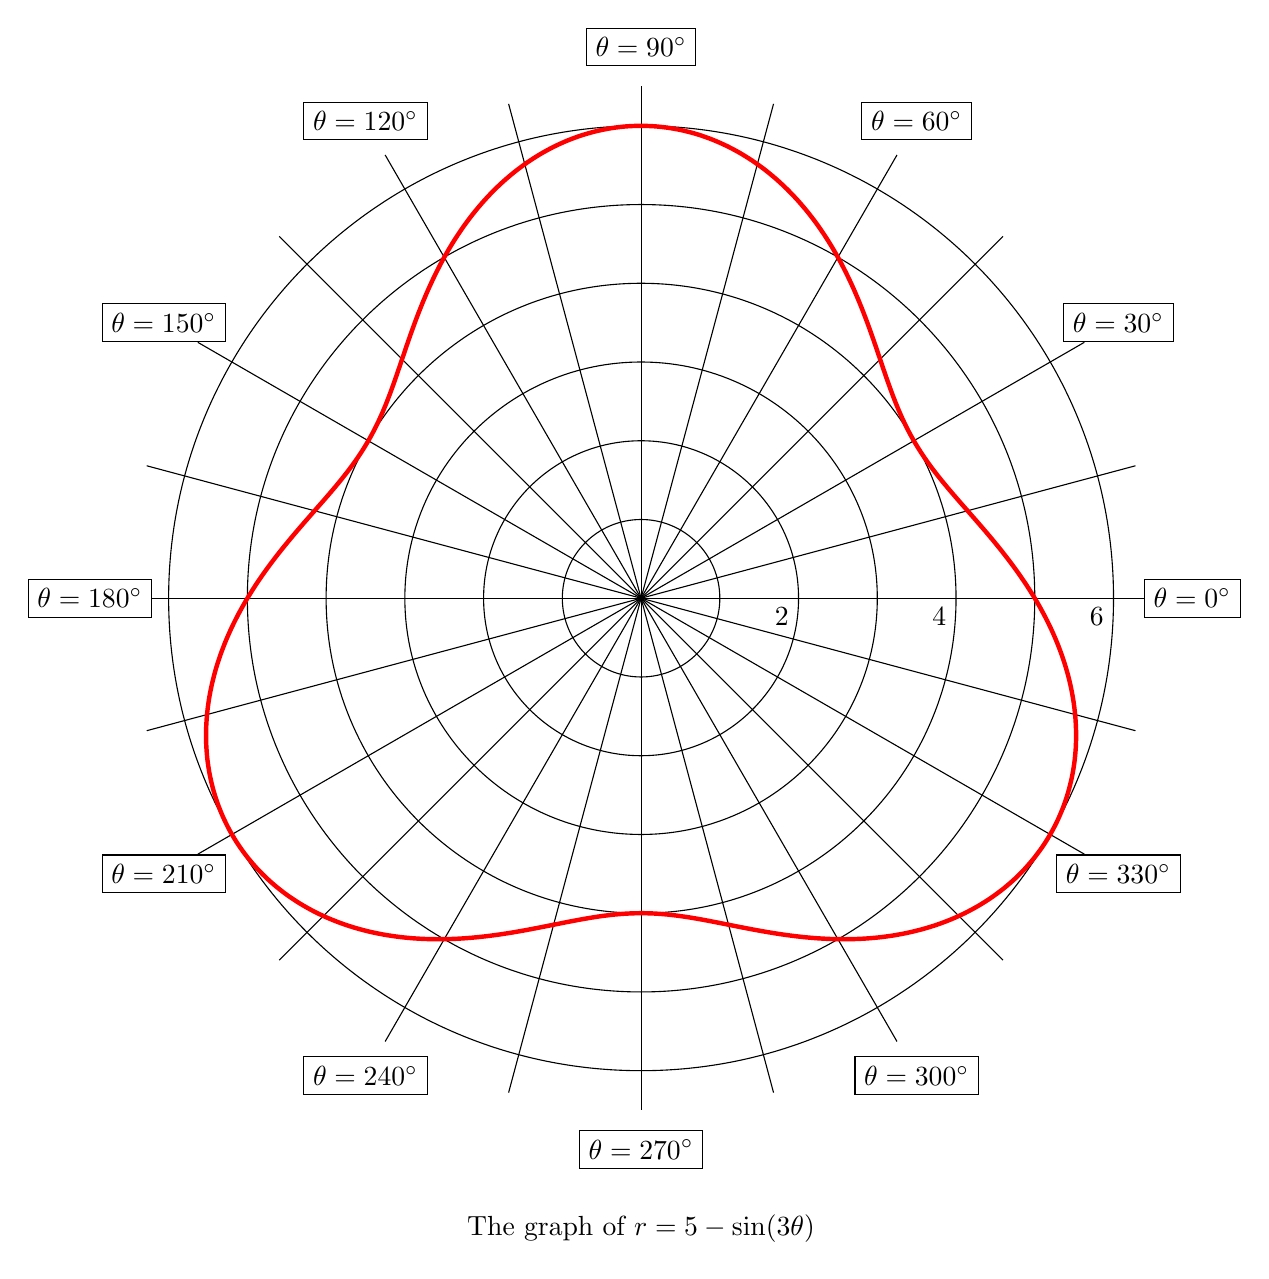
\begin{tikzpicture}
  % drawing grid lines
  \foreach \r in {1,...,6} {\draw (0,0) circle (\r);}
  \draw (-6.5,0) -- (6.5,0);
  \foreach \theta in {15,30,...,165} {\draw (\theta:6.5) -- (\theta+180:6.5);}
  % labelling them
  \foreach \r in {2,4,6} {\node[below left] (lbl\r) at (\r,0) {\r};}
  \foreach \t in {0,30,...,330} {
    \node [draw,fill=white] (lbl\t) at (\t:7) {$\theta = \t^\circ$};
  }
  % graph of $r = 5 - \sin(3\theta)$
  \draw[red,ultra thick,smooth cycle,samples=200,domain=0:359]
  plot (\x:{5-sin(3*\x)});
  \node at (270:8) {The graph of $r = 5 - \sin(3\theta)$};
\end{tikzpicture}
\end{document}
